% Options for packages loaded elsewhere
\PassOptionsToPackage{unicode}{hyperref}
\PassOptionsToPackage{hyphens}{url}
\PassOptionsToPackage{dvipsnames,svgnames,x11names}{xcolor}
%
\documentclass[
  authoryear,
  preprint,
  3p,
  twocolumn]{elsarticle}

\usepackage{amsmath,amssymb}
\usepackage{iftex}
\ifPDFTeX
  \usepackage[T1]{fontenc}
  \usepackage[utf8]{inputenc}
  \usepackage{textcomp} % provide euro and other symbols
\else % if luatex or xetex
  \usepackage{unicode-math}
  \defaultfontfeatures{Scale=MatchLowercase}
  \defaultfontfeatures[\rmfamily]{Ligatures=TeX,Scale=1}
\fi
\usepackage{lmodern}
\ifPDFTeX\else  
    % xetex/luatex font selection
\fi
% Use upquote if available, for straight quotes in verbatim environments
\IfFileExists{upquote.sty}{\usepackage{upquote}}{}
\IfFileExists{microtype.sty}{% use microtype if available
  \usepackage[]{microtype}
  \UseMicrotypeSet[protrusion]{basicmath} % disable protrusion for tt fonts
}{}
\makeatletter
\@ifundefined{KOMAClassName}{% if non-KOMA class
  \IfFileExists{parskip.sty}{%
    \usepackage{parskip}
  }{% else
    \setlength{\parindent}{0pt}
    \setlength{\parskip}{6pt plus 2pt minus 1pt}}
}{% if KOMA class
  \KOMAoptions{parskip=half}}
\makeatother
\usepackage{xcolor}
\setlength{\emergencystretch}{3em} % prevent overfull lines
\setcounter{secnumdepth}{5}
% Make \paragraph and \subparagraph free-standing
\makeatletter
\ifx\paragraph\undefined\else
  \let\oldparagraph\paragraph
  \renewcommand{\paragraph}{
    \@ifstar
      \xxxParagraphStar
      \xxxParagraphNoStar
  }
  \newcommand{\xxxParagraphStar}[1]{\oldparagraph*{#1}\mbox{}}
  \newcommand{\xxxParagraphNoStar}[1]{\oldparagraph{#1}\mbox{}}
\fi
\ifx\subparagraph\undefined\else
  \let\oldsubparagraph\subparagraph
  \renewcommand{\subparagraph}{
    \@ifstar
      \xxxSubParagraphStar
      \xxxSubParagraphNoStar
  }
  \newcommand{\xxxSubParagraphStar}[1]{\oldsubparagraph*{#1}\mbox{}}
  \newcommand{\xxxSubParagraphNoStar}[1]{\oldsubparagraph{#1}\mbox{}}
\fi
\makeatother

\usepackage{color}
\usepackage{fancyvrb}
\newcommand{\VerbBar}{|}
\newcommand{\VERB}{\Verb[commandchars=\\\{\}]}
\DefineVerbatimEnvironment{Highlighting}{Verbatim}{commandchars=\\\{\}}
% Add ',fontsize=\small' for more characters per line
\usepackage{framed}
\definecolor{shadecolor}{RGB}{241,243,245}
\newenvironment{Shaded}{\begin{snugshade}}{\end{snugshade}}
\newcommand{\AlertTok}[1]{\textcolor[rgb]{0.68,0.00,0.00}{#1}}
\newcommand{\AnnotationTok}[1]{\textcolor[rgb]{0.37,0.37,0.37}{#1}}
\newcommand{\AttributeTok}[1]{\textcolor[rgb]{0.40,0.45,0.13}{#1}}
\newcommand{\BaseNTok}[1]{\textcolor[rgb]{0.68,0.00,0.00}{#1}}
\newcommand{\BuiltInTok}[1]{\textcolor[rgb]{0.00,0.23,0.31}{#1}}
\newcommand{\CharTok}[1]{\textcolor[rgb]{0.13,0.47,0.30}{#1}}
\newcommand{\CommentTok}[1]{\textcolor[rgb]{0.37,0.37,0.37}{#1}}
\newcommand{\CommentVarTok}[1]{\textcolor[rgb]{0.37,0.37,0.37}{\textit{#1}}}
\newcommand{\ConstantTok}[1]{\textcolor[rgb]{0.56,0.35,0.01}{#1}}
\newcommand{\ControlFlowTok}[1]{\textcolor[rgb]{0.00,0.23,0.31}{\textbf{#1}}}
\newcommand{\DataTypeTok}[1]{\textcolor[rgb]{0.68,0.00,0.00}{#1}}
\newcommand{\DecValTok}[1]{\textcolor[rgb]{0.68,0.00,0.00}{#1}}
\newcommand{\DocumentationTok}[1]{\textcolor[rgb]{0.37,0.37,0.37}{\textit{#1}}}
\newcommand{\ErrorTok}[1]{\textcolor[rgb]{0.68,0.00,0.00}{#1}}
\newcommand{\ExtensionTok}[1]{\textcolor[rgb]{0.00,0.23,0.31}{#1}}
\newcommand{\FloatTok}[1]{\textcolor[rgb]{0.68,0.00,0.00}{#1}}
\newcommand{\FunctionTok}[1]{\textcolor[rgb]{0.28,0.35,0.67}{#1}}
\newcommand{\ImportTok}[1]{\textcolor[rgb]{0.00,0.46,0.62}{#1}}
\newcommand{\InformationTok}[1]{\textcolor[rgb]{0.37,0.37,0.37}{#1}}
\newcommand{\KeywordTok}[1]{\textcolor[rgb]{0.00,0.23,0.31}{\textbf{#1}}}
\newcommand{\NormalTok}[1]{\textcolor[rgb]{0.00,0.23,0.31}{#1}}
\newcommand{\OperatorTok}[1]{\textcolor[rgb]{0.37,0.37,0.37}{#1}}
\newcommand{\OtherTok}[1]{\textcolor[rgb]{0.00,0.23,0.31}{#1}}
\newcommand{\PreprocessorTok}[1]{\textcolor[rgb]{0.68,0.00,0.00}{#1}}
\newcommand{\RegionMarkerTok}[1]{\textcolor[rgb]{0.00,0.23,0.31}{#1}}
\newcommand{\SpecialCharTok}[1]{\textcolor[rgb]{0.37,0.37,0.37}{#1}}
\newcommand{\SpecialStringTok}[1]{\textcolor[rgb]{0.13,0.47,0.30}{#1}}
\newcommand{\StringTok}[1]{\textcolor[rgb]{0.13,0.47,0.30}{#1}}
\newcommand{\VariableTok}[1]{\textcolor[rgb]{0.07,0.07,0.07}{#1}}
\newcommand{\VerbatimStringTok}[1]{\textcolor[rgb]{0.13,0.47,0.30}{#1}}
\newcommand{\WarningTok}[1]{\textcolor[rgb]{0.37,0.37,0.37}{\textit{#1}}}

\providecommand{\tightlist}{%
  \setlength{\itemsep}{0pt}\setlength{\parskip}{0pt}}\usepackage{longtable,booktabs,array}
\usepackage{calc} % for calculating minipage widths
% Correct order of tables after \paragraph or \subparagraph
\usepackage{etoolbox}
\makeatletter
\patchcmd\longtable{\par}{\if@noskipsec\mbox{}\fi\par}{}{}
\makeatother
% Allow footnotes in longtable head/foot
\IfFileExists{footnotehyper.sty}{\usepackage{footnotehyper}}{\usepackage{footnote}}
\makesavenoteenv{longtable}
\usepackage{graphicx}
\makeatletter
\def\maxwidth{\ifdim\Gin@nat@width>\linewidth\linewidth\else\Gin@nat@width\fi}
\def\maxheight{\ifdim\Gin@nat@height>\textheight\textheight\else\Gin@nat@height\fi}
\makeatother
% Scale images if necessary, so that they will not overflow the page
% margins by default, and it is still possible to overwrite the defaults
% using explicit options in \includegraphics[width, height, ...]{}
\setkeys{Gin}{width=\maxwidth,height=\maxheight,keepaspectratio}
% Set default figure placement to htbp
\makeatletter
\def\fps@figure{htbp}
\makeatother

\makeatletter
\@ifpackageloaded{caption}{}{\usepackage{caption}}
\AtBeginDocument{%
\ifdefined\contentsname
  \renewcommand*\contentsname{Table of contents}
\else
  \newcommand\contentsname{Table of contents}
\fi
\ifdefined\listfigurename
  \renewcommand*\listfigurename{List of Figures}
\else
  \newcommand\listfigurename{List of Figures}
\fi
\ifdefined\listtablename
  \renewcommand*\listtablename{List of Tables}
\else
  \newcommand\listtablename{List of Tables}
\fi
\ifdefined\figurename
  \renewcommand*\figurename{Figure}
\else
  \newcommand\figurename{Figure}
\fi
\ifdefined\tablename
  \renewcommand*\tablename{Table}
\else
  \newcommand\tablename{Table}
\fi
}
\@ifpackageloaded{float}{}{\usepackage{float}}
\floatstyle{ruled}
\@ifundefined{c@chapter}{\newfloat{codelisting}{h}{lop}}{\newfloat{codelisting}{h}{lop}[chapter]}
\floatname{codelisting}{Listing}
\newcommand*\listoflistings{\listof{codelisting}{List of Listings}}
\makeatother
\makeatletter
\makeatother
\makeatletter
\@ifpackageloaded{caption}{}{\usepackage{caption}}
\@ifpackageloaded{subcaption}{}{\usepackage{subcaption}}
\makeatother
\usepackage{float}
\makeatletter
\let\oldlt\longtable
\let\endoldlt\endlongtable
\def\longtable{\@ifnextchar[\longtable@i \longtable@ii}
\def\longtable@i[#1]{\begin{figure}[H]
\onecolumn
\begin{minipage}{0.5\textwidth}
\oldlt[#1]
}
\def\longtable@ii{\begin{figure}[H]
\onecolumn
\begin{minipage}{0.5\textwidth}
\oldlt
}
\def\endlongtable{\endoldlt
\end{minipage}
\twocolumn
\end{figure}}
\makeatother
\journal{Escuela Nacional de Estudios Superiores Unidad Mérida, UNAM}

\ifLuaTeX
  \usepackage{selnolig}  % disable illegal ligatures
\fi
\usepackage[]{natbib}
\bibliographystyle{elsarticle-harv}
\usepackage{bookmark}

\IfFileExists{xurl.sty}{\usepackage{xurl}}{} % add URL line breaks if available
\urlstyle{same} % disable monospaced font for URLs
\hypersetup{
  pdftitle={Monitoreo del estado ecológico de una playa representativa de la península de Yucatán para tres grupos clave},
  pdfauthor={Ricardo De La Rosa-Castillo; Darío Q. Gutiérrez-Urrutia; Elian G. Vivas-Camacho},
  pdfkeywords={keyword1, keyword2},
  colorlinks=true,
  linkcolor={blue},
  filecolor={Maroon},
  citecolor={Blue},
  urlcolor={Blue},
  pdfcreator={LaTeX via pandoc}}


\setlength{\parindent}{6pt}
\begin{document}

\begin{frontmatter}
\title{Monitoreo del estado ecológico de una playa representativa de la
península de Yucatán para tres grupos clave}
\author[]{Ricardo De La Rosa-Castillo%
\corref{cor1}%
}
 \ead{319296972@gmail.com} 
\author[]{Darío Q. Gutiérrez-Urrutia%
%
}
 \ead{bob@example.com} 
\author[]{Elian G. Vivas-Camacho%
%
}
 \ead{cat@example.com} 


\cortext[cor1]{Corresponding author}



        
\begin{abstract}
This is the abstract. Lorem ipsum dolor sit amet, consectetur adipiscing
elit. Vestibulum augue turpis, dictum non malesuada a, volutpat eget
velit. Nam placerat turpis purus, eu tristique ex tincidunt et. Mauris
sed augue eget turpis ultrices tincidunt. Sed et mi in leo porta
egestas. Aliquam non laoreet velit. Nunc quis ex vitae eros aliquet
auctor nec ac libero. Duis laoreet sapien eu mi luctus, in bibendum leo
molestie. Sed hendrerit diam diam, ac dapibus nisl volutpat vitae.
Aliquam bibendum varius libero, eu efficitur justo rutrum at. Sed at
tempus elit.
\end{abstract}





\begin{keyword}
    keyword1 \sep 
    keyword2
\end{keyword}
\end{frontmatter}
    

\section{Introducción}\label{introducciuxf3n}

Las playas en la Península de Yucatán son zonas esenciales para la
biodiversidad regional y global, no sólo porque funcionan como refugio
para especies de animales migratorios de importancia mundial, sino
también porque son hábitat para especies clave, fundamentales en el
flujo de energía en las redes tróficas y de interacción entre los
organismos de los ecosistemas. Más allá de su belleza, las playas
yucatecas deben preservarse para garantizar la sostenibilidad y el
bienestar de las comunidades costeras y marinas
\citep{AguilarMedrano2007}.

Una demostración de lo anterior son las comunidades de pastos marinos
que cubren las costas poco profundas de la península. En estas grandes
extensiones de vegetación se encuentran siete de las once especies que
hay en México de estas plantas acuáticas, \emph{Thalassia testudinum}
König 1805, \emph{Halodule wrightii} Ascherson 1868, \emph{Syringodium
filiforme} Kützing 1860, \emph{Halophila engelmannii} Ascherson 1875,
\emph{Halophila decipiens} Ostenfeld 1902, \emph{Ruppia maritima}
Linnaeus 1753 y \emph{Ruppia mexicana} den Hartog \& van Tussenbroek
2016 \citep{EspinozaAvalos1996, DENHARTOG201638}.

Las comunidades de estas plantas actúan como captadores de carbono
masivos, reteniendo entre 48 y 112 Tg de carbono al año, incluyendo el
carbono en la biomasa de estos organismos y los sedimentos que retienen
como reservorio \citep{Kennedy2010, OCANA2023102979}. Este reservorio se
mantiene gracias al dosel foliar y a su sistema radical, los cuales
funcionan como trampas de sedimentos \citep{Fourqurean2012}. Además, los
pastos marinos son disipadores de la energía de las corrientes, lo que
evita que el sedimento se mantenga suspendido en la columna de agua.
Estas características y funciones ecológicas dependen tanto de la
composición de las comunidades, como de la morfología y fisiología de
las especies \citep{GarciaDuarte2001}; lo anterior vuelve fundamental
llevar a cabo un monitoreo constante de estas zonas.

Los pastos marinos también proporcionan refugio y alimento a diversas
especies de animales. De todos, destacamos particularmente a los peces,
cuya presencia y abundancia refleja salud en las comunidades. Comprender
esta relación resulta muy valioso para la conservación de estas zonas.
Así, el monitoreo de las poblaciones de peces en las zonas de pastos
marinos resulta una muy buena herramienta para evaluar el equilibrio
ecológico, ya que, de observar cambios en su distribución, es posible
indicar alteraciones en la capacidad de los pastos marinos para retener
carbono y mantener la estabilidad de la comunidad
\citep{AguilarMedrano2007, CHOVANEC2003639}.

De la misma manera, las plantas y los peces no son los únicos grupos
cuya presencia puede indicar alteraciones en la salud de la comunidad.
La subclase Oligochaeta (Annelida) es un grupo de gusanos que forma
parte de la meiofauna marina y que cumple un papel fundamental en la
estabilidad del sistema costero al ser parte esencial de las redes
tróficas como alimento de diversas especies de animales, incluidos peces
\citep{Diaz1987}. Además, este grupo edáfico contribuye al reciclaje de
la materia orgánica y a la oxigenación en el sedimento; lo que influye
directamente en la calidad del agua y suelo en las playas
\citep{Giere2006, Verdonschot2001, Collado1999}.

En este grupo de organismos, \emph{Tubificoides diazi} Brinkhurst \&
Baker 1979 destaca por su gran abundancia en los suelos arenosos de las
playas de Yucatán, ofreciendo la oportunidad de analizar la abundancia y
estructura de las poblaciones de oligoquetos para observar el estado de
salud del agua, del suelo y la sostenibilidad de la zona en general
\citep{behrend_takeda_gomes_fernandes_2012}. Esto resalta la importancia
de su monitoreo como bioindicadores ecológicos.

Dada la importancia de pastos marinos, peces y oligoquetos en la
estabilidad ecológica de las playas de la península de Yucatán, una
serie de muestreos que integren a estos tres grupos puede resultar
valiosa para el monitoreo de áreas de conservación. Destacamos la
importancia de emplear protocolos de muestreo existentes, ya que es
fundamental para presentar información comparable con estudios previos y
posteriores al presente, lo que permitirá obtener una perspectiva más
completa del estado ecológico de la zona. Así, el objetivo de este
trabajo es reportar el estado ecológico actual de una playa
representativa de la península de Yucatán a partir del análisis de la
composición y estructura de las comunidades de pastos marinos, de peces
y de la estructura de la población de oligoquetos.

Se plantean las siguientes hipótesis: (1) en zonas más someras existirá
un mayor desarrollo de pastos marinos y algas en comparación a zonas más
hondas, explicado por una disminución en la cantidad de luz disponible;
(2) la composición diversa de la pradera de pastos marinos que
proporciona hábitat, junto con la presencia de \emph{T. diazi} como
recurso alimenticio, fomentan la presencia de distintas especies de
peces; (3) la población de \emph{T. diazi} se concentrará en la zona
intermareal, ya que esta ofrece un refugio contra la depredación por
parte de peces en la zona submareal, mientras que evitan la desecación
asociada a la zona supramareal.

A partir de las hipótesis anteriores, se espera observar en
profundidades someras en comparación con profundidades más hondas: (1)
Una mayor cobertura de pastos marinos y un mayor número de especies; (2)
mayor biomasa en peso húmedo de algas; (3) mayor número de haces
foliares y de vástagos de pastos marinos; (4) marcas de herbivoría
visibles en pastos marinos; (5) un mayor largo de individuos de pastos
marinos; (6) mayor biomasa en peso húmedo de pastos marinos. Además,
esperamos observar (7) el mismo número de especies de peces reportadas
en muestreos similares anteriormente en el sitio y, por último, (8) un
mayor número de individuos de \emph{T. diazi} en la zona intermareal en
comparación con las zonas supramareal y submareal.

\section{Materiales y métodos}\label{materiales-y-muxe9todos}

\subsection{\texorpdfstring{\textbf{Área de
estudio}}{Área de estudio}}\label{uxe1rea-de-estudio}

El presente se llevó a cabo en Dzilam de Bravo (21.390166° N, 88.908361°
W), región costera del norte de la península de Yucatán, México. Este
sitio fue seleccionado debido a su diversidad ecológica, la cual incluye
a los grupos objeto de estudio. La zona se caracteriza por un clima
cálido a lo largo del año, con temperaturas promedio anuales de 25.3 °C.
El sustrato predominante en la zona es arena fina.

\subsection{\texorpdfstring{\textbf{Muestreo}}{Muestreo}}\label{muestreo}

\subsubsection{Parámetros
fisicoquímicos}\label{paruxe1metros-fisicoquuxedmicos}

Se midieron parámetros fisicoquímicos del agua marina de la zona dos
veces al día, entre las 7:00 y las 11:00 hrs (matutino), y entre las
15:00 y las 18:00 hrs (vespertino), en dos días distintos separados por
un día, tomando como referencia el muelle con las coordenadas 21.39027°
N, 88.90837° W. Para este procedimiento se utilizó un medidor
multiparamétrico ProQuatro YSI, el cual ofrece valores en tiempo real
de: oxígeno disuelto (OD) (mg/L), salinidad (ppt), sólidos disueltos
totales (SDT) (mg/L), pH, temperatura (C°), entre otros parámetros. Los
mencionados son aquellos que se registraron para el presente estudio.

\subsubsection{Abundancia relativa}\label{abundancia-relativa}

La metodología empleada en este apartado se basa en la propuesta por
\citet{Botello2022} como `Indicador 3'. Se seleccionaron cuatro sitios
de muestreo dentro de un área de 5 metros de radio. Después, en cada uno
de los sitios se colocó una unidad de muestreo (UM), la cual se trataba
de un cuadrante de 1 m2 hecho de tubo PVC, dividido en 16 cuadrados con
hilo de nailon, subunidades de muestreo (SUM), donde cada una de estas
representó el 6.25\% de la UM. Empleando una cámara acuática Nikon W300,
se tomaron fotografías de cada una de las SUM para ser procesadas
posteriormente en el laboratorio de campo, únicamente cuando las
partículas de sedimento suspendidas en el agua no comprometían el
análisis de los grupos presentes en la imagen; de ser el caso contrario,
se registraron la presencia y proporciones (en porcentaje) de los grupos
\emph{in situ}.

En ambos casos, las proporciones se obtuvieron por determinación visual.
De igual manera, se destaca la importancia de inspeccionar entre los
haces de los pastos para verificar la presencia de taxones de menor
tamaño. Toda esta metodología se llevó a cabo en los horarios matutino y
vespertino definidos anteriormente en dos días separados por un día.
Para el primer día, el procedimiento se llevó a cabo en una zona somera
para el horario matutino y en una zona profunda para el horario
vespertino; para el segundo día, se llevó a cabo en una zona profunda
para el horario matutino y en una zona somera para el horario
vespertino.

\subsubsection{Biomasa de macroalgas}\label{biomasa-de-macroalgas}

La metodología empleada en este apartado se basa en la propuesta por
\citet{Botello2022} como `Indicador 4'. Se seleccionaron dos sitios de
muestreo, separados por 5 metros, distintos a los del procedimiento
anterior. En la UM, que es la misma que se utiliza en el protocolo
anterior, seleccionamos una de las SUM para colectar todos los cuerpos
de macroalgas presentes en él; cuando fue posible, se separaron del
sedimento que pudieran retener. Esta metodología se llevó a cabo en los
horarios, días y profundidades definidas en el protocolo anterior. Las
muestras de cada sitio se separaron por morfotipos distintos para
después ser identificadas al menor nivel taxonómico posible con base en
la guía de \citet{Littler1989}. Por último, cada grupo identificado fue
pesado en húmedo.

\subsubsection{Pastos marinos}\label{pastos-marinos}

La metodología empleada en este apartado se basa en las propuestas por
\citet{Botello2022} como `Indicador 5', `Indicador 6' e `Indicador 7'.
Se seleccionaron dos sitios de muestreo, separados por 5 metros,
distintos a los del procedimiento anterior, estos sitios caracterizados
uno como representativo de la diversidad de la zona y otro de mayor
abundancia de pastos marinos. Después, en cada sitio se extrajo un
núcleo de sedimento y vegetación empleando una herramienta apropiada
para esto, de 15 cm de diámetro y 30 cm de alto, acomodando las hojas
largas de los pastos marinos bajo la herramienta. Del núcleo extraído se
conservaron los organismos y se regresó el sedimento de la muestra al
lugar del que fue extraído para mitigar el efecto del muestreo en la
comunidad. Esta metodología se llevó a cabo en los horarios, días y
profundidades definidas anteriormente.

Las muestras obtenidas se procesaron en el laboratorio de campo. Se
pesaron las muestras obtenidas para cada grupo de pasto y macroalgas;
sin embargo, en pastos se separaron los tejidos de arriba del sedimento
y los de abajo del sedimento, en la medida de lo posible, y se pesaron
ambas partes resultantes por separado para cada grupo de pasto. Además,
a cada pasto marino se le contó el número de haces foliares, se buscó la
presencia de marcas de herbivoría y, por último, se midieron los tres
individuos más largos.

\subsubsection{Peces}\label{peces}

La metodología empleada en este apartado se basa en la propuesta por
\citet{Botello2022} como `Indicador 11'. Se seleccionaron dos sitios en
zonas despejadas sin vegetación. Debido a que la presencia de humanos
ahuyenta a los peces de los pastizales, se usaron cámaras para
fotografiar y grabar a los peces en la zona. En el primer sitio se
posicionaron dos cámaras encontradas para que tomaran fotografías cada
dos minutos durante 24 horas. En el segundo sitio se colocaron cuatro
cámaras dispuestas en los puntos cardinales para grabar durante 1 hora.
Tras recuperar las cámaras, se analizó el material obtenido para
identificar las especies de peces con base en la guía de
\citet{Gallardo-Torres2014}.

\subsubsection{Oligoquetos}\label{oligoquetos}

El suelo donde se tomaron las muestras presentó, para el gradiente de la
zona supramareal a la submareal, variaciones en la textura y/o en la
cobertura de biomasa, sin embargo, se mantuvo consistente en estas
composiciones para las réplicas. El muestreo se realizó en tres días,
con un día de separación entre cada uno. El primer muestreo se llevó a
cabo en horario vespertino, el segundo en horarios matutino y
vespertino, y el último sólo en horario matutino. Los horarios se
definieron a las 6:00 horas para matutino y a las 15:00 horas para
vespertino. Se realizaron en transectos, separados por 50 metros, cada
uno partiendo de la zona del rompimiento de olas (intermareal) hacia la
zona supramareal y la zona submareal.

El punto intermareal se estableció por la tarde para el primer día y por
la mañana para el segundo y tercero, el punto intermareal se mantuvo en
el mismo lugar para la medición en el horario de la tarde del segundo
día, además, desde el punto intermareal se midió la distancia a un punto
de referencia, donde terminara la línea de playa y comenzara la
vegetación de duna costera.

Para la extracción de núcleos de suelo se utilizó una herramienta
cilíndrica de 30 cm de diámetro y 50 cm de altura. Los núcleos se
tomaron con una separación de un metro entre cada uno. Se realizaron un
total de ocho transectos, cada uno con nueve núcleos, cuatro en la zona
supramareal, cuatro en la submareal y uno en la intermareal. Los gusanos
fueron extraídos mediante un proceso de tamizado en el que el sustrato
se lavó tres veces con agua agitada para facilitar la salida de los
organismos. Después, se separaron en frascos con agua marina recolectada
en el sitio. En el laboratorio de campo, se contó el número de
individuos extraídos de cada núcleo y se midió la talla de cada
organismo en centímetros de largo.

\subsection{\texorpdfstring{\textbf{Análisis de
datos}}{Análisis de datos}}\label{anuxe1lisis-de-datos}

Los datos obtenidos en campo, se almacenaron en hojas de cálculo para su
posterior análisis. Todo el análisis se realizó en R (4.3.1) utilizando
RStudio (2024.4.0.735). Las pruebas estadísticas se realizaron de manera
independiente para los distintos conjuntos de datos obtenidos.

Para los datos obtenidos del protocolo de oligoquetos, se tenía planeado
comparar la abundancia y talla entre las distintas regiones de la playa
(submareal, intermareal, supramareal) sin embargo, al empezar a extraer
los oligoquetos se volvió aparente que existe más variación dentro, que
entre las distintas regiones de la playa (ver \citet{fig1}), por lo que
se decidió tratar los distintos núcleos como unidades de muestreo
separadas.

Previo al análisis estadístico se realizaron pruebas Shapiro-Wilks y
Levene \{car\}, para observar la distribución de los datos y la
homogeneidad de varianza. Dado que tanto los datos de talla de
oligoquetos como su abundancia, no cumplieron los supuestos para un
Análisis de Varianza, se optó por realizar un análisis de varianza
multivariante permutacional (PERMANOVA). Antes de ejecutar el PERMANOVA
los datos se transformaron mediante una raíz cuarta para reducir la
influencia de los valores extremos.

El PERMANOVA se realizó utilizando una matriz de distancia euclidiana,
tanto para los datos de talla, como los de abundancia. La cantidad de
oligoquetos medidos limitó el número de permutaciones a 99. Para el
análisis de abundancia se logró realizar 9,999 permutaciones. Para ambos
análisis se midió el efecto de dos factores: el horario de la medición,
y la posición de la playa.

Dada la naturaleza del estudio de cobertura de pastos marinos y algas,
se ejecutó un PERMANOVA. Se empezó agrupando los datos de cobertura de
las SUM, y convirtiéndolos en porcentajes. Al igual que con el análisis
de oligoquetos los datos se transformaron con una raíz cuarta.
Posteriormente se generó una matriz de distancia Bray-Curtis, antes de
realizar un PERMANOVA, de 9,999 permutaciones, utilizando como factor la
profundidad categórica. El peso de algas colectadas de los
cuadrantes,asi como el de las algas y pastos extraídos con el nucleador,
fue analizado de la misma manera. Por último, se realizaron dos
PERMANOVAs utilizando matrices de distancias euclidianas analizando, el
número de haces y el tamaño de las especies de pastos marinos extraídos
con el nucleador.

\section{Resultados}\label{resultados}

\begin{figure}[H]

{\centering \includegraphics[width=0.5\textwidth,height=\textheight]{ECVI_files/figure-pdf/fig1-1.pdf}

}

\caption{Tamaño de Oligoquetos en los distintos horarios}

\end{figure}%

\begin{figure}[H]

{\centering 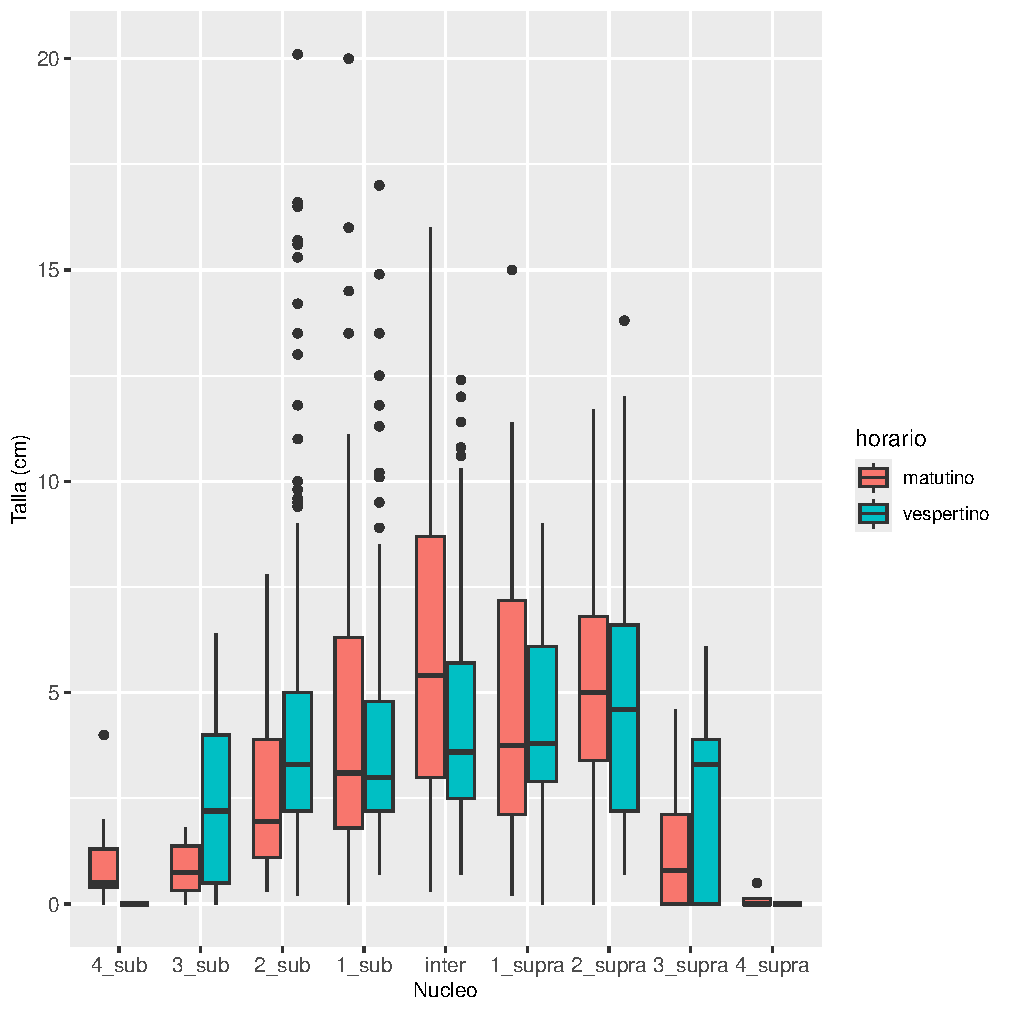
\includegraphics[width=0.5\textwidth,height=\textheight]{ECVI_files/figure-pdf/Fig2-1.pdf}

}

\caption{Talla de oligoquetos en los núcleos}

\end{figure}%

\section{Bibliography styles}\label{bibliography-styles}

Here are two sample references: \citet{Feynman1963118}
\citet{Dirac1953888}.

With this template using elsevier class, natbib will be used. Three
bibliographic style files (*.bst) are provided and their use controled by
\texttt{cite-style} option:

\begin{itemize}
\tightlist
\item
  \texttt{citestyle:\ number} (default) will use
  \texttt{elsarticle-num.bst} - can be used for the numbered scheme
\item
  \texttt{citestyle:\ numbername} will use
  \texttt{elsarticle-num-names.bst} - can be used for numbered with new
  options of natbib.sty
\item
  \texttt{citestyle:\ authoryear} will use \texttt{elsarticle-harv.bst}
  --- can be used for author year scheme
\end{itemize}

This \texttt{citestyle} will insert the right \texttt{.bst} and set the
correct \texttt{classoption} for \texttt{elsarticle} document class.

Using \texttt{natbiboptions} variable in YAML header, you can set more
options for \texttt{natbib} itself . Example

\begin{Shaded}
\begin{Highlighting}[]
\FunctionTok{natbiboptions}\KeywordTok{:}\AttributeTok{ longnamesfirst,angle,semicolon}
\end{Highlighting}
\end{Shaded}

\subsection{Using CSL}\label{using-csl}

If \texttt{cite-method} is set to \texttt{citeproc} in
\texttt{elsevier\_article()}, then pandoc is used for citations instead
of \texttt{natbib}. In this case, the \texttt{csl} option is used to
format the references. By default, this template will provide an
appropriate style, but alternative \texttt{csl} files are available from
\url{https://www.zotero.org/styles?q=elsevier}. These can be downloaded
and stored locally, or the url can be used as in the example header.

\section{Equations}\label{equations}

Here is an equation: \[ 
  f_{X}(x) = \left(\frac{\alpha}{\beta}\right)
  \left(\frac{x}{\beta}\right)^{\alpha-1}
  e^{-\left(\frac{x}{\beta}\right)^{\alpha}}; 
  \alpha,\beta,x > 0 .
\]

Inline equations work as well: \(\sum_{i = 2}^\infty\{\alpha_i^\beta\}\)

\section{Figures and tables}\label{figures-and-tables}

Figure~\ref{fig-meaningless} is generated using an R chunk.

\begin{figure}

\centering{

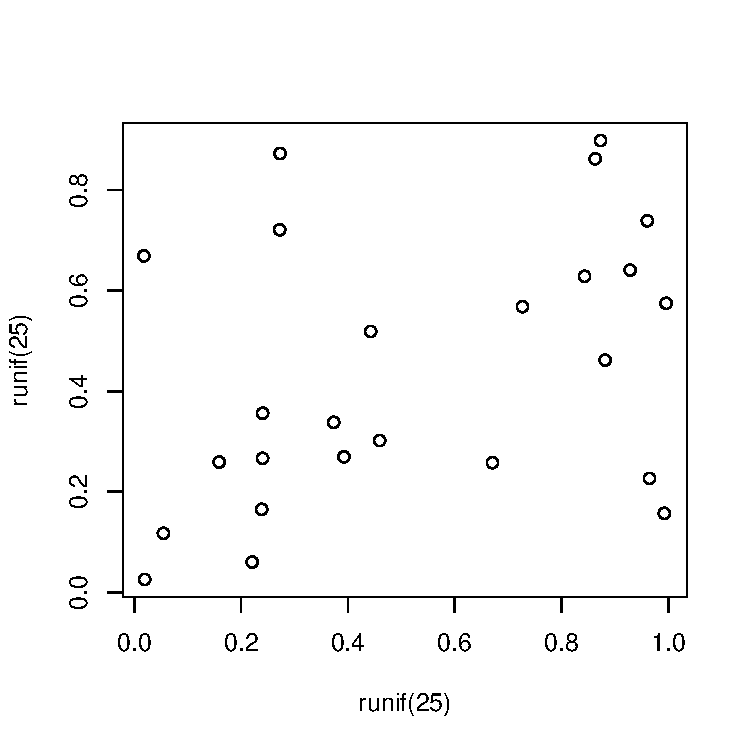
\includegraphics[width=0.5\textwidth,height=\textheight]{ECVI_files/figure-pdf/fig-meaningless-1.pdf}

}

\caption{\label{fig-meaningless}A meaningless scatterplot}

\end{figure}%

\section{Tables coming from R}\label{tables-coming-from-r}

Tables can also be generated using R chunks, as shown in
Table~\ref{tbl-simple} example.

\begin{Shaded}
\begin{Highlighting}[]
\NormalTok{knitr}\SpecialCharTok{::}\FunctionTok{kable}\NormalTok{(}\FunctionTok{head}\NormalTok{(mtcars)[,}\DecValTok{1}\SpecialCharTok{:}\DecValTok{4}\NormalTok{])}
\end{Highlighting}
\end{Shaded}

\begin{longtable}[]{@{}lrrrr@{}}

\caption{\label{tbl-simple}Caption centered above table}

\tabularnewline

\toprule\noalign{}
& mpg & cyl & disp & hp \\
\midrule\noalign{}
\endhead
\bottomrule\noalign{}
\endlastfoot
Mazda RX4 & 21.0 & 6 & 160 & 110 \\
Mazda RX4 Wag & 21.0 & 6 & 160 & 110 \\
Datsun 710 & 22.8 & 4 & 108 & 93 \\
Hornet 4 Drive & 21.4 & 6 & 258 & 110 \\
Hornet Sportabout & 18.7 & 8 & 360 & 175 \\
Valiant & 18.1 & 6 & 225 & 105 \\

\end{longtable}


\renewcommand\refname{Referencias}
  \bibliography{bibliography.bib}



\end{document}
